\documentclass[12pt]{article}
%\usepackage[latin1]{inputenc}
\usepackage[utf8]{inputenc}
\usepackage{float}
\usepackage{amsmath,amsfonts}
\usepackage{graphicx}
\usepackage[authoryear]{natbib}
\usepackage{xr}
\externaldocument{cs_texas}
\usepackage[unicode=true]
 {hyperref}
%\usepackage{breakurl}

\usepackage{array}

\usepackage[centerlast,bf,justification=justified,singlelinecheck=false]{caption}
\usepackage{graphicx}
\usepackage[table]{xcolor}
\usepackage{multirow}
\usepackage{hhline}
\usepackage{calc} 
\usepackage{tabularx}
\usepackage{booktabs}  
\usepackage[flushleft]{threeparttable}
\usepackage{pdflscape}

\usepackage[title]{appendix}

\usepackage{tikz}
\usetikzlibrary{decorations.pathreplacing}

%\setlength\labelsep{0pt}

%%%%%%%%%%%%%%%%%%%%%%%%%%%%%%  PACKAGES FOR COMMENTING
% THIS ADDS TEXT BOXES IN THE MARGIN
\usepackage[colorinlistoftodos,textsize=small]{todonotes}

% IF SELECTED, COMMAND WILL NOT DISPLAY COMMENTED TEXT  
%\newcommand{\comment}[1]{}  %comment not shown

%IF SELECTED, COMMAND WILL PRINT COMMENTED TEXT IN BLUE  
\newcommand{\comment}[1]
{{\bfseries \color{red} #1}} %comment shown

\newcommand{\inputy}[1]{\input{#1}\unskip}

%%%%%%%%%%%%%%%%%%%%%%%%%%%%%% User specified LaTeX commands.

\oddsidemargin 0in \evensidemargin 0in \topmargin 0in \columnsep 10pt
\columnseprule 0pt \marginparwidth 90pt \marginparsep 11pt
\marginparpush 5pt \headheight 0pt \headsep 0pt \textheight 9in
\textwidth 6.5in

\usepackage{setspace}
\usepackage{xcolor}
\hypersetup{
    colorlinks,
    linkcolor={blue!80!black},
    citecolor={blue!80!black},
    urlcolor={blue!80!black}
}

%THIS ALLOWS US TO HIDE FACT DRAFT WAS COMPILED THE DAY OF SUBMISSION 
\usepackage{datetime2,datetime2-calc}
\DTMnewdatestyle{Myyyy}{%
  \renewcommand*{\DTMdisplaydate}[4]{\DTMmonthname{##2}~##1}%
  \renewcommand*{\DTMDisplaydate}{\DTMdisplaydate}%
}
\DTMsetdatestyle{Myyyy}

% Ryan Kellogg's custom figure note function
\DeclareTextFontCommand{\fignotefont}{\normalfont\footnotesize}
\newcommand{\fignote}[2][\linewidth]{
    \begin{minipage}[]{#1}
        \vspace{12pt}
        \fignotefont{#2}
    \end{minipage}}

\makeatletter

%COMBINE MULTIPLE TABLES IN A FLOAT	
\usepackage[position=top]{subfig}
\captionsetup{position=top}

%\@ifundefined{showcaptionsetup}{}{%
%	\PassOptionsToPackage{caption=false}{subfig}}
%\usepackage{subfig}
%\makeatother

%\renewcommand{\thesection}{\Roman{section}} 

%%%%%%%%%%%%%%%%%%%%%%%%%%%%%% END PREAMBLE %%%%%%%%%%%%%%%%%%%%%%%%%%%%%% 

\begin{document}

\title{Online Appendix For \\ ``Relinquishing Riches: \\ Auctions vs Informal Negotiations \\ in Texas Oil and Gas Leasing''
\thanks{Both authors declare they have no interests, financial or otherwise, that relate to the research described in this paper, nor do they have any current ties, directly or indirectly to the energy industry. We thank participants at numerous seminars, as well as Steve Cicala, Piotr Dworczak, Aaron Flaaen, Timothy Fitzgerald, Ryan Kellogg, Peter Maniloff, and Cythina Lin Lawell for helpful comments.  Yixin Sun, Eric Karsten, Devin McNulty and Grace Park provided excellent research assistance. Code for replication available at \href{https://github.com/rlsweeney/public_cs_texas}{https://github.com/rlsweeney/public\_cs\_texas}.}
\vspace{10pt}}

\author{Thomas R. Covert \thanks{University of Chicago Booth School of Business and NBER, \protect\href{mailto:Thomas.Covert@chicagobooth.edu}{Thomas.Covert@chicagobooth.edu}.}
\\
 Richard L. Sweeney \thanks{Boston College, \protect\href{mailto:sweeneri@bc.edu}{sweeneri@bc.edu}.}}

\date{\today \\
 \vspace{0.5cm}
}
\maketitle

\setcounter{page}{1} \onehalfspace

\newpage

\begin{appendices}

\section{Additional Tables and Figures}

\setcounter{figure}{0}  \renewcommand{\thefigure}{A.\arabic{figure}} 
\setcounter{table}{0}  \renewcommand{\thetable}{A.\arabic{table}} 

\subsection{RAL vs State Lease Locations}
\begin{figure}[H]
\begin{centering}
\caption{Map of Sample Leases by Type \label{fig:RAL_map}}
\vspace{-10pt}
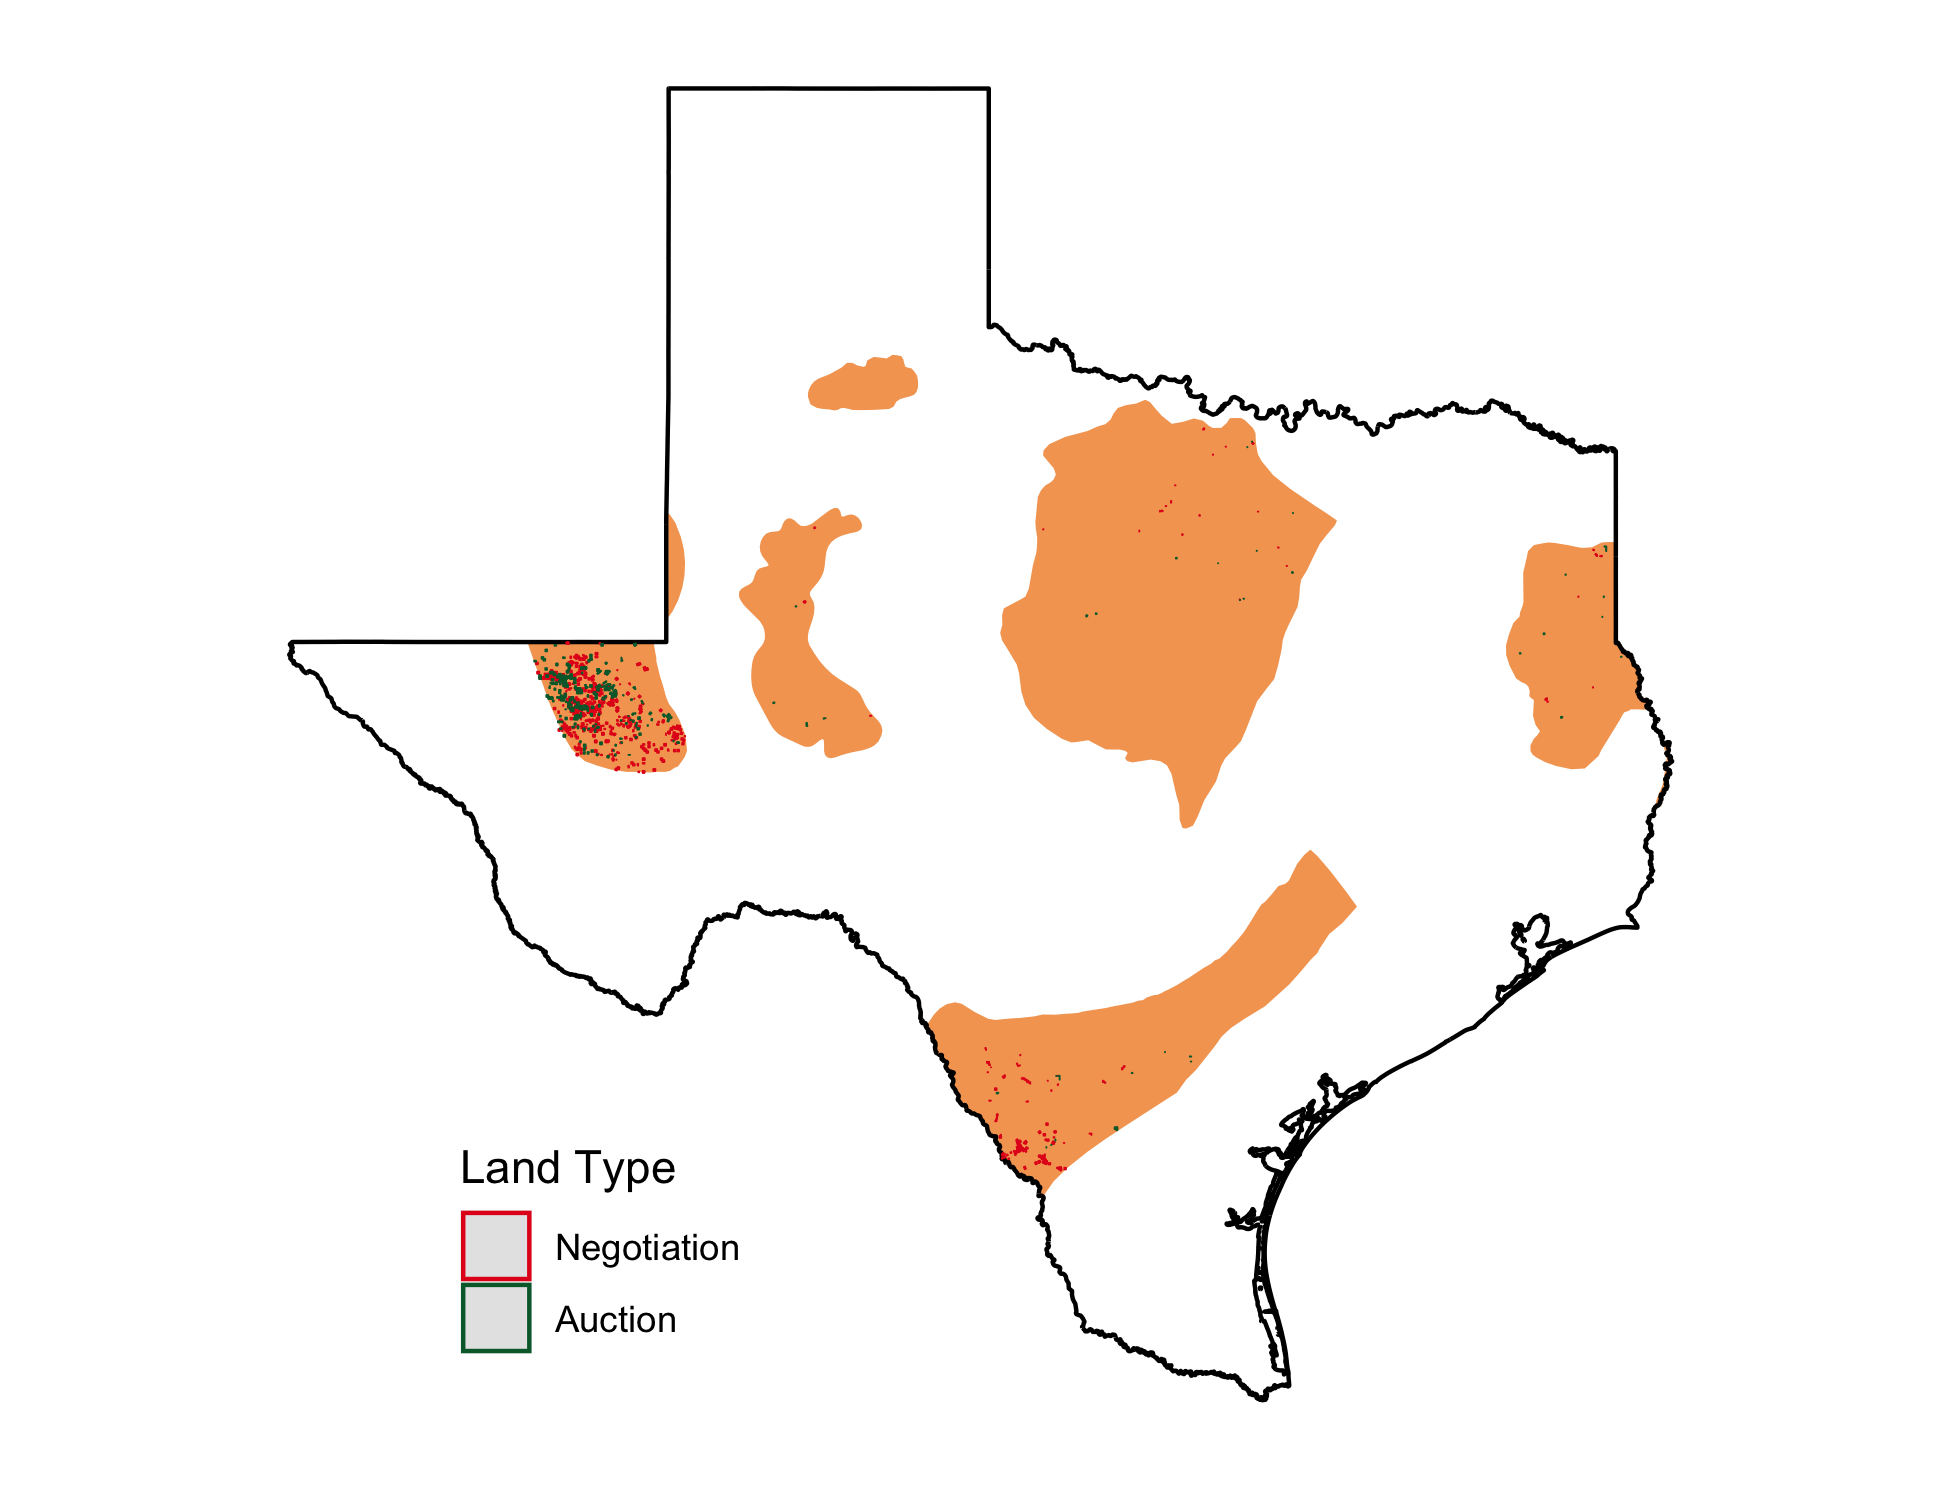
\includegraphics[width=1\textwidth]{../output/figures/glo_leases_in_texas.png}
\par\end{centering}
\end{figure}

\subsection{Additional Lease Results}\label{sec:extra_regressions}

%\addtolength{\tabcolsep}{6pt}
\begin{table}[H]
	\begin{center}
	\begin{threeparttable}
		\caption{Bonus Payments and Mechanism Type, per Acre}
		\label{tab:table_main_bonus_levels}
		\small
		
\begin{tabular}{lccccccccc}
\toprule
 & ( 1 ) & ( 2 ) & ( 3 ) & ( 4 ) & ( 5 ) & ( 6 ) & ( 7 ) & ( 8 ) & ( 9 )\\
\midrule
 & 0.63 & 0.66 & 0.82 & 0.64 & 0.78 & 0.66 & 0.77 & 0.87 & 1.06\\

\multirow{-2}{*}{\raggedright\arraybackslash Auction} & (0.14) & (0.18) & (0.28) & (0.19) & (0.11) & (0.19) & (0.10) & (0.34) & (0.19)\\

\midrule
Grid & 10 & 10 & 10 & 20 & DML & 10 & DML & 10 & DML\\

Time & Q & GY,Q & GYQ & GY,Q & DML & GY,Q & DML & GY,Q & DML\\

Extra & No & No & No & No & No & Yes & Yes & No & No\\

Private Only & No & No & No & No & No & No & No & Yes & Yes\\

N & 1,515 & 1,515 & 1,515 & 1,515 & 1,515 & 1,260 & 1,260 & 1,308 & 1,308\\

$R^2$ & 0.728 & 0.880 & 0.901 & 0.807 &  & 0.868 &  & 0.890 & \\
\bottomrule
\end{tabular}
            
		\begin{tablenotes}
		\footnotesize
		\item The dependent variable in each regression is the the lease's bonus payment per acre. In columns 1-4, the size of the location bins, in miles, are indicated in the ``Grid'' row, while the structure of the time controls (``Q'' for quarter of sample, ``GY,Q'' for grid-by-year plus quarter of sample, and ``GYQ'' for grid-by-quarter of sample) are indicated in the ``Time'' row.  Standard errors are clustered by grid in columns 1-4.  Column 5 uses a double/debiased machine learning routine, as recommended in \cite{chernozhukov2018double}.  Fixed effect models include a spline in lease size while the DML model includes lease size as a random forest covariates.  
		\end{tablenotes}
	\end{threeparttable}
	\end{center}
\end{table}



\addtolength{\tabcolsep}{-4pt}
\begin{table}[H]
	\begin{center}
	\begin{threeparttable}
	\caption{Lease Bonus Regressions with Controls for Royalty Rate and Term}
	\label{tab:BonusWithRoyaltyTerm}
	\small
	
\begin{tabular}{lcccccc}
\toprule
 & ( 1 ) & ( 2 ) & ( 3 ) & ( 4 ) & ( 5 ) & ( 6 )\\
\midrule
 & 0.72 & 0.68 & 0.96 & 0.43 & 0.43 & 0.57\\

\multirow{-2}{*}{\raggedright\arraybackslash Auction} & (0.18) & (0.16) & (0.13) & (0.06) & (0.05) & (0.05)\\

\midrule
Estimate & G10Y & G20Y & DML & G10Y & G20Y & DML\\

Outcome & Bonus per acre & Bonus per acre & Bonus per acre & log(Bonus) & log(Bonus) & log(Bonus)\\
\midrule

N & 1,515 & 1,515 & 1,515 & 1,515 & 1,515 & 1,515\\
\bottomrule
\end{tabular}
            
		\begin{tablenotes}
		\footnotesize
		\item The dependent variable is either bonus per acre (in thousands per acre) or the natural logarithm of the bonus payment.  The Grid10-Year and Grid20-Year fixed-effect specifications include a spline in lease acreage and linear terms for term length and royalty rate, while the DML specifications include these variables as  random forest covariates.     
		\end{tablenotes}	   
	\end{threeparttable}
	\end{center}
\end{table}

\begin{table}[H]
	\begin{center}
	\begin{threeparttable}
	\caption{Lease Output Regressions with Controls for Royalty Rate and Term}
	\label{tab:OutputWithRoyaltyTerm}
	\small
	
\begin{tabular}{lcccccc}
\toprule
  & ( 1 ) & ( 2 ) & ( 3 ) & ( 4 ) & ( 5 ) & ( 6 )\\
\midrule
 & 3.85 & 4.44 & 6.14 & 0.53 & 0.77 & 0.75\\

\multirow{-2}{*}{\raggedright\arraybackslash Auction - Lease Revenue} & (1.46) & (1.54) & (1.90) & (0.20) & (0.22) & (0.08)\\

N & 1,259 & 1,259 & 1,259 & 746 & 980 & \vphantom{1} 1,259\\

\midrule
 & 1.17 & 1.32 & 1.55 & 0.62 & 0.83 & 0.81\\

\multirow{-2}{*}{\raggedright\arraybackslash Auction - Output} & (0.41) & (0.41) & (0.43) & (0.21) & (0.25) & (0.24)\\

N & 1,259 & 1,259 & 1,259 & 746 & 980 & 1,259\\

\midrule
 & 1.31 & 1.56 & 2.16 & 0.48 & 0.65 & 0.84\\

\multirow{-2}{*}{\raggedright\arraybackslash Auction - Seller Revenue} & (0.39) & (0.39) & (0.49) & (0.12) & (0.14) & (0.23)\\

N & 1,259 & 1,259 & 1,259 & 1,259 & 1,259 & 1,259\\

\midrule
Estimate & G10Y & G20Y & DML & G10Y & G20Y & DML\\

Estimator & Linear & Linear & Linear & Poisson & Poisson & Poisson\\
\bottomrule
\end{tabular}
            
		\begin{tablenotes}
		\footnotesize
		\item The dependent variables are per-acre (lease and seller revenue in thousands per acre, output in hundreds of BOE per acre) in the linear specifications and in aggregate (not per acre) in the Poisson specifications.  The Grid10-Year and Grid20-Year fixed-effect specifications include a spline in lease acreage and linear terms for term length and royalty rate, while the DML specifications include these variables as  random forest covariates.    
		\end{tablenotes}	   
	\end{threeparttable}
	\end{center}
\end{table}

\addtolength{\tabcolsep}{10pt}
\begin{table}[H]
	\begin{center}
	\begin{threeparttable}
		\caption{Drilled Regressions}\label{tab:drilledregs}
		 \small
			 
\begin{tabular}{lccccc}
\toprule
 & ( 1 ) & ( 2 ) & ( 3 ) & ( 4 ) & ( 5 )\\
\midrule
 & 0.07 & 0.05 & 0.08 & 0.07 & 0.04\\

\multirow{-2}{*}{\raggedright\arraybackslash Auction} & (0.03) & (0.04) & (0.06) & (0.03) & (0.03)\\

\midrule
Grid & 10 & 10 & 10 & 20 & DML\\

Time & Q & GY,Q & GYQ & GY,Q & DML\\

N & 1,259 & 1,259 & 1,259 & 1,259 & 1,259\\

$R^2$ & 0.375 & 0.626 & 0.719 & 0.489 & \\
\bottomrule
\end{tabular}
            
			\footnotesize
			\begin{tablenotes}
				\item The dependent variable is equal to 1 if a lease was drilled during its primary term and 0 otherwise.  The sample includes all leases whose primary term ends before March, 2019.  In columns 1-4, the size of the location bins, in miles, are indicated in the ``Grid'' row, while the structure of the time controls (``Q'' for quarter of sample, ``GY,Q'' for grid-by-year plus quarter of sample, and ``GYQ'' for grid-by-quarter of sample) are indicated in the ``Time'' row.  Standard errors are clustered by grid in columns 1-4.  Column 5 uses a double/debiased machine learning routine.  Fixed effect models include a spline in lease size and the DML model includes lease size as a random forest covariate.
			\end{tablenotes} 
	\end{threeparttable}
	\end{center}
\end{table}
	
	\begin{table}[H]
	\begin{center}
	\begin{threeparttable}
		\caption{Log Output Regressions Among the Sample of Leases That Are Drilled}\label{tab:outputconddrilled}
		 \small
			 
\begin{tabular}{lccccc}
\toprule
 & ( 1 ) & ( 2 ) & ( 3 ) & ( 4 ) & ( 5 )\\
\midrule
 & 0.40 & 0.52 & 0.33 & 0.58 & 0.45\\

\multirow{-2}{*}{\raggedright\arraybackslash Auction} & (0.19) & (0.20) & (0.25) & (0.22) & (0.17)\\

\midrule
Grid & 10 & 10 & 10 & 20 & DML\\

Time & Q & GY,Q & GYQ & GY,Q & DML\\

N & 425 & 425 & 425 & 425 & 425\\

$R^2$ & 0.652 & 0.856 & 0.909 & 0.774 & \\
\bottomrule
\end{tabular}
            
			\footnotesize
			\begin{tablenotes}
				\item The dependent variable is the natural logarithm of discounted barrels of oil equivalent (Output) per acre.  The sample includes all drilled leases whose primary term ends before March, 2019.  In columns 1-4, the size of the location bins, in miles, are indicated in the ``Grid'' row, while the structure of the time controls (``Q'' for quarter of sample, ``GY,Q'' for grid-by-year plus quarter of sample, and ``GYQ'' for grid-by-quarter of sample) are indicated in the ``Time'' row.  Standard errors are clustered by grid in columns 1-4.  Column 5 uses a double/debiased machine learning routine.  Fixed effect models include a spline in lease size and the DML model includes lease size as a random forest covariate.
			\end{tablenotes} 
	\end{threeparttable}
	\end{center}
\end{table}
\addtolength{\tabcolsep}{-10pt}

\subsection{Unleased Spell Duration Analysis}\label{app:duration}
Our lease and parcel data make it possible to reliably identify which parcels have active leases starting in January, 2001.  We leases to their parcels using our existing parcel-lease map and then merge this with our lease revenue data, which starts in January, 2001.  We define a lease as active during a given month if that month is during the lease's primary term or if that month is spanned by the earliest and latest royalty payments we observe for the lease.  We say a lease is terminated at the later of a lease's primary term expiration and its last observed royalty payment.  If a given terminated lease is the only lease currently active in a parcel, we say that parcel is \textit{unleased} at that point.  As soon as another lease is signed that is associated with a parcel, we say the parcel as \textit{leased} again.  With this structure, every parcel in our data is either leased or unleased on January 1, 2001, and for every subsequent month, and we use this parcel-by-month panel to construct ``unleased spells'' for every parcel.  It is worth noting that parcels which are unleased as of January 1, 2001 may have been unleased previous to this point.  As a result, unleased spells that begin in January, 2001 may be left-censored.  

In the unleased spell analyses that follow, we define four samples of unleased spells.  The ``All'' spell sample is everything described above, while the ``First'' spell sample is just the first unleased spell for each parcel.  The ``Uncensored'' spell sample excludes unleased spells that begin in January, 2001, because we do not know whether they began earlier than January 2001 or not.  Finally, the ``First Uncensored'' spell sample is the first uncensored unleased spell for each parcel.  Table \ref{tab:SpellDefs} tabulates how many spells we have under each of these definitions, for RAL and State parcels, starting in each year between 2001 and 2019.

\begin{table}[htbp]
	\begin{center}
		\begin{threeparttable}
			\caption{Parcel Unleased Spell Counts}\label{tab:SpellDefs}
			\label{tab:summary_stats}
			\small
			
\begin{tabular}{rrrrrrrrr}
\toprule
\multicolumn{1}{c}{ } & \multicolumn{2}{c}{All} & \multicolumn{2}{c}{Uncensored} & \multicolumn{2}{c}{First} & \multicolumn{2}{c}{First Uncensored} \\
\cmidrule(l{3pt}r{3pt}){2-3} \cmidrule(l{3pt}r{3pt}){4-5} \cmidrule(l{3pt}r{3pt}){6-7} \cmidrule(l{3pt}r{3pt}){8-9}
Year & RAL & State & RAL & State & RAL & State & RAL & State\\
\midrule
2001 & 1439 & 450 & 17 & 10 & 1439 & 450 & 17 & 10\\
2002 & 20 & 1 & 20 & 1 & 20 & 1 & 20 & 1\\
2003 & 234 & 61 & 234 & 61 & 233 & 61 & 233 & 61\\
2004 & 72 & 4 & 72 & 4 & 59 & 4 & 72 & 4\\
2005 & 22 & 5 & 22 & 5 & 10 & 5 & 19 & 5\\
2006 & 24 & 10 & 24 & 10 & 2 & 1 & 21 & 10\\
2007 & 36 & 2 & 36 & 2 & 1 & 1 & 31 & 2\\
2008 & 57 & 1 & 57 & 1 & 4 & 0 & 44 & 1\\
2009 & 162 & 23 & 162 & 23 & 8 & 2 & 67 & 15\\
2010 & 163 & 89 & 163 & 89 & 2 & 2 & 138 & 58\\
2011 & 62 & 25 & 62 & 25 & 1 & 0 & 43 & 23\\
2012 & 46 & 10 & 46 & 10 & 4 & 0 & 30 & 7\\
2013 & 78 & 10 & 78 & 10 & 1 & 0 & 47 & 10\\
2014 & 37 & 2 & 37 & 2 & 0 & 0 & 19 & 1\\
2015 & 44 & 17 & 44 & 17 & 1 & 2 & 16 & 8\\
2016 & 106 & 58 & 106 & 58 & 2 & 4 & 16 & 24\\
2017 & 97 & 8 & 97 & 8 & 1 & 2 & 33 & 7\\
2018 & 77 & 10 & 77 & 10 & 1 & 0 & 31 & 5\\
2019 & 18 & 13 & 18 & 13 & 3 & 0 & 6 & 0\\
\bottomrule
\end{tabular}

			\footnotesize
			\begin{tablenotes}
				\item ``All'' refers to all unleased spells on on-shale PSF parcels since January 1, 2001.  ``Uncensored'' spells are the subset of those parcels which were already leased on January 1, 2001.  The date at which these spells begin is thus uncensored.  ``First'' spells are the subset of all spells which are the first unleased spell for a given parcel, and ``First Uncensored'' spells are the subset of uncensored spells which are the first unleased, uncensored spell for a given parcel.
			\end{tablenotes}
		\end{threeparttable}
	\end{center}
\end{table}

Our first test of the hypothesis that RAL and State parcels experience differentially long unleased spells makes use of the adjusted Kaplan-Meier survival curve estimator, derived in \cite{xie2005adjusted}.  This estimate of  survival curves is similar to traditional ``unadjusted'' non-parametric survival curve estimate in experimental data, with the main difference being that each observation is weighted by the inverse of a propensity score.  Here we estimate the probability that a spell on a parcel in a given location, of a given size, at a given point in time, is on an RAL or State parcel using a fixed-effects logit model, with Grid-by-year and Year-by-quarter fixed effects, as well as a spline in parcel acres.  Letting $\widehat{p}_i$ be the estimated propensity score for spell $i$, we assign a weight of $\frac{1}{\widehat{p}_i}$ to spells on State parcels, and a weight of $\frac{1}{1-\widehat{p}_i}$ to RAL parcels.  As described above, we estimate these survival curves under four different samples of unleased spells, as shown in figures \ref{fig:km10} and \ref{fig:km20}.\footnote{We use the \texttt{ipw.survival} command from the R language package \texttt{RISCA}.}  Under both 10-mile and 20-mile grid fixed effects, as well as all four sample definitions, there is no visual difference in ``survival'' between the two samples.  Unleased spells on State and RAL parcels seem to end equally quickly.

\begin{figure}[H]
	\centering
	\caption{Covariate-Adjusted Kaplan-Meier Survival Curves: Grid 10 Specifications}\label{fig:km10}
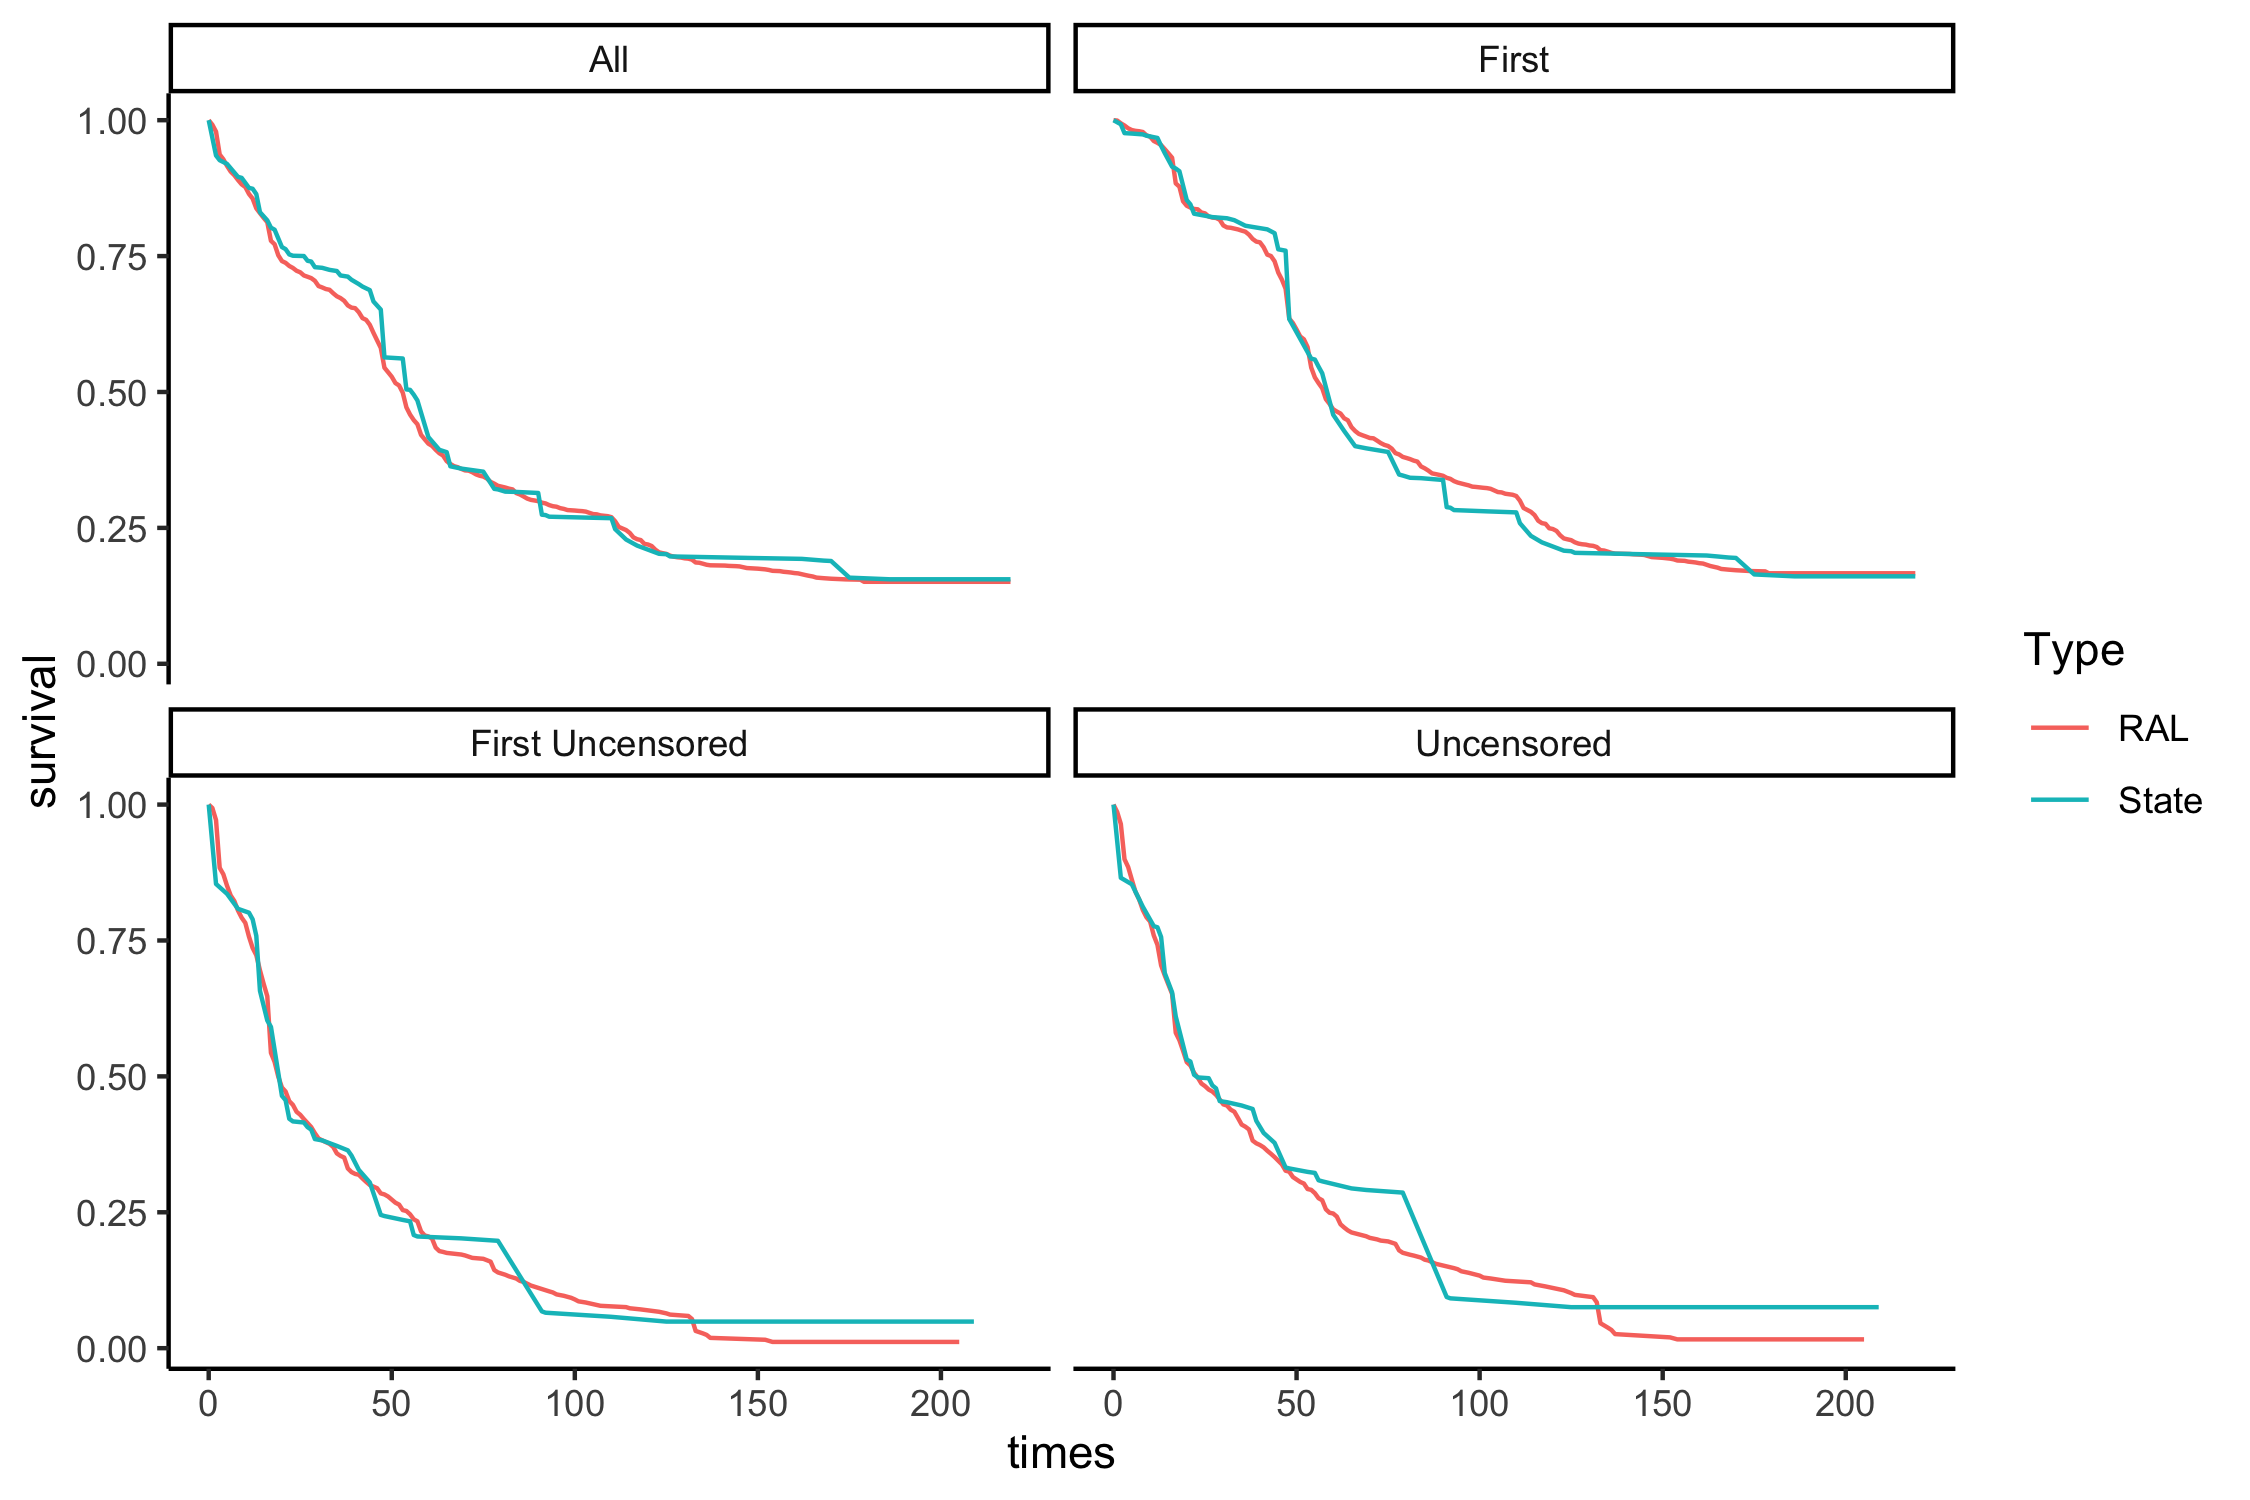
\includegraphics[width=1\textwidth]{../output/figures/ipwkm10.png}
\end{figure}

\begin{figure}[H]
	\centering
	\caption{Covariate-Adjusted Kaplan-Meier Survival Curves: Grid 20 Specifications}\label{fig:km20}
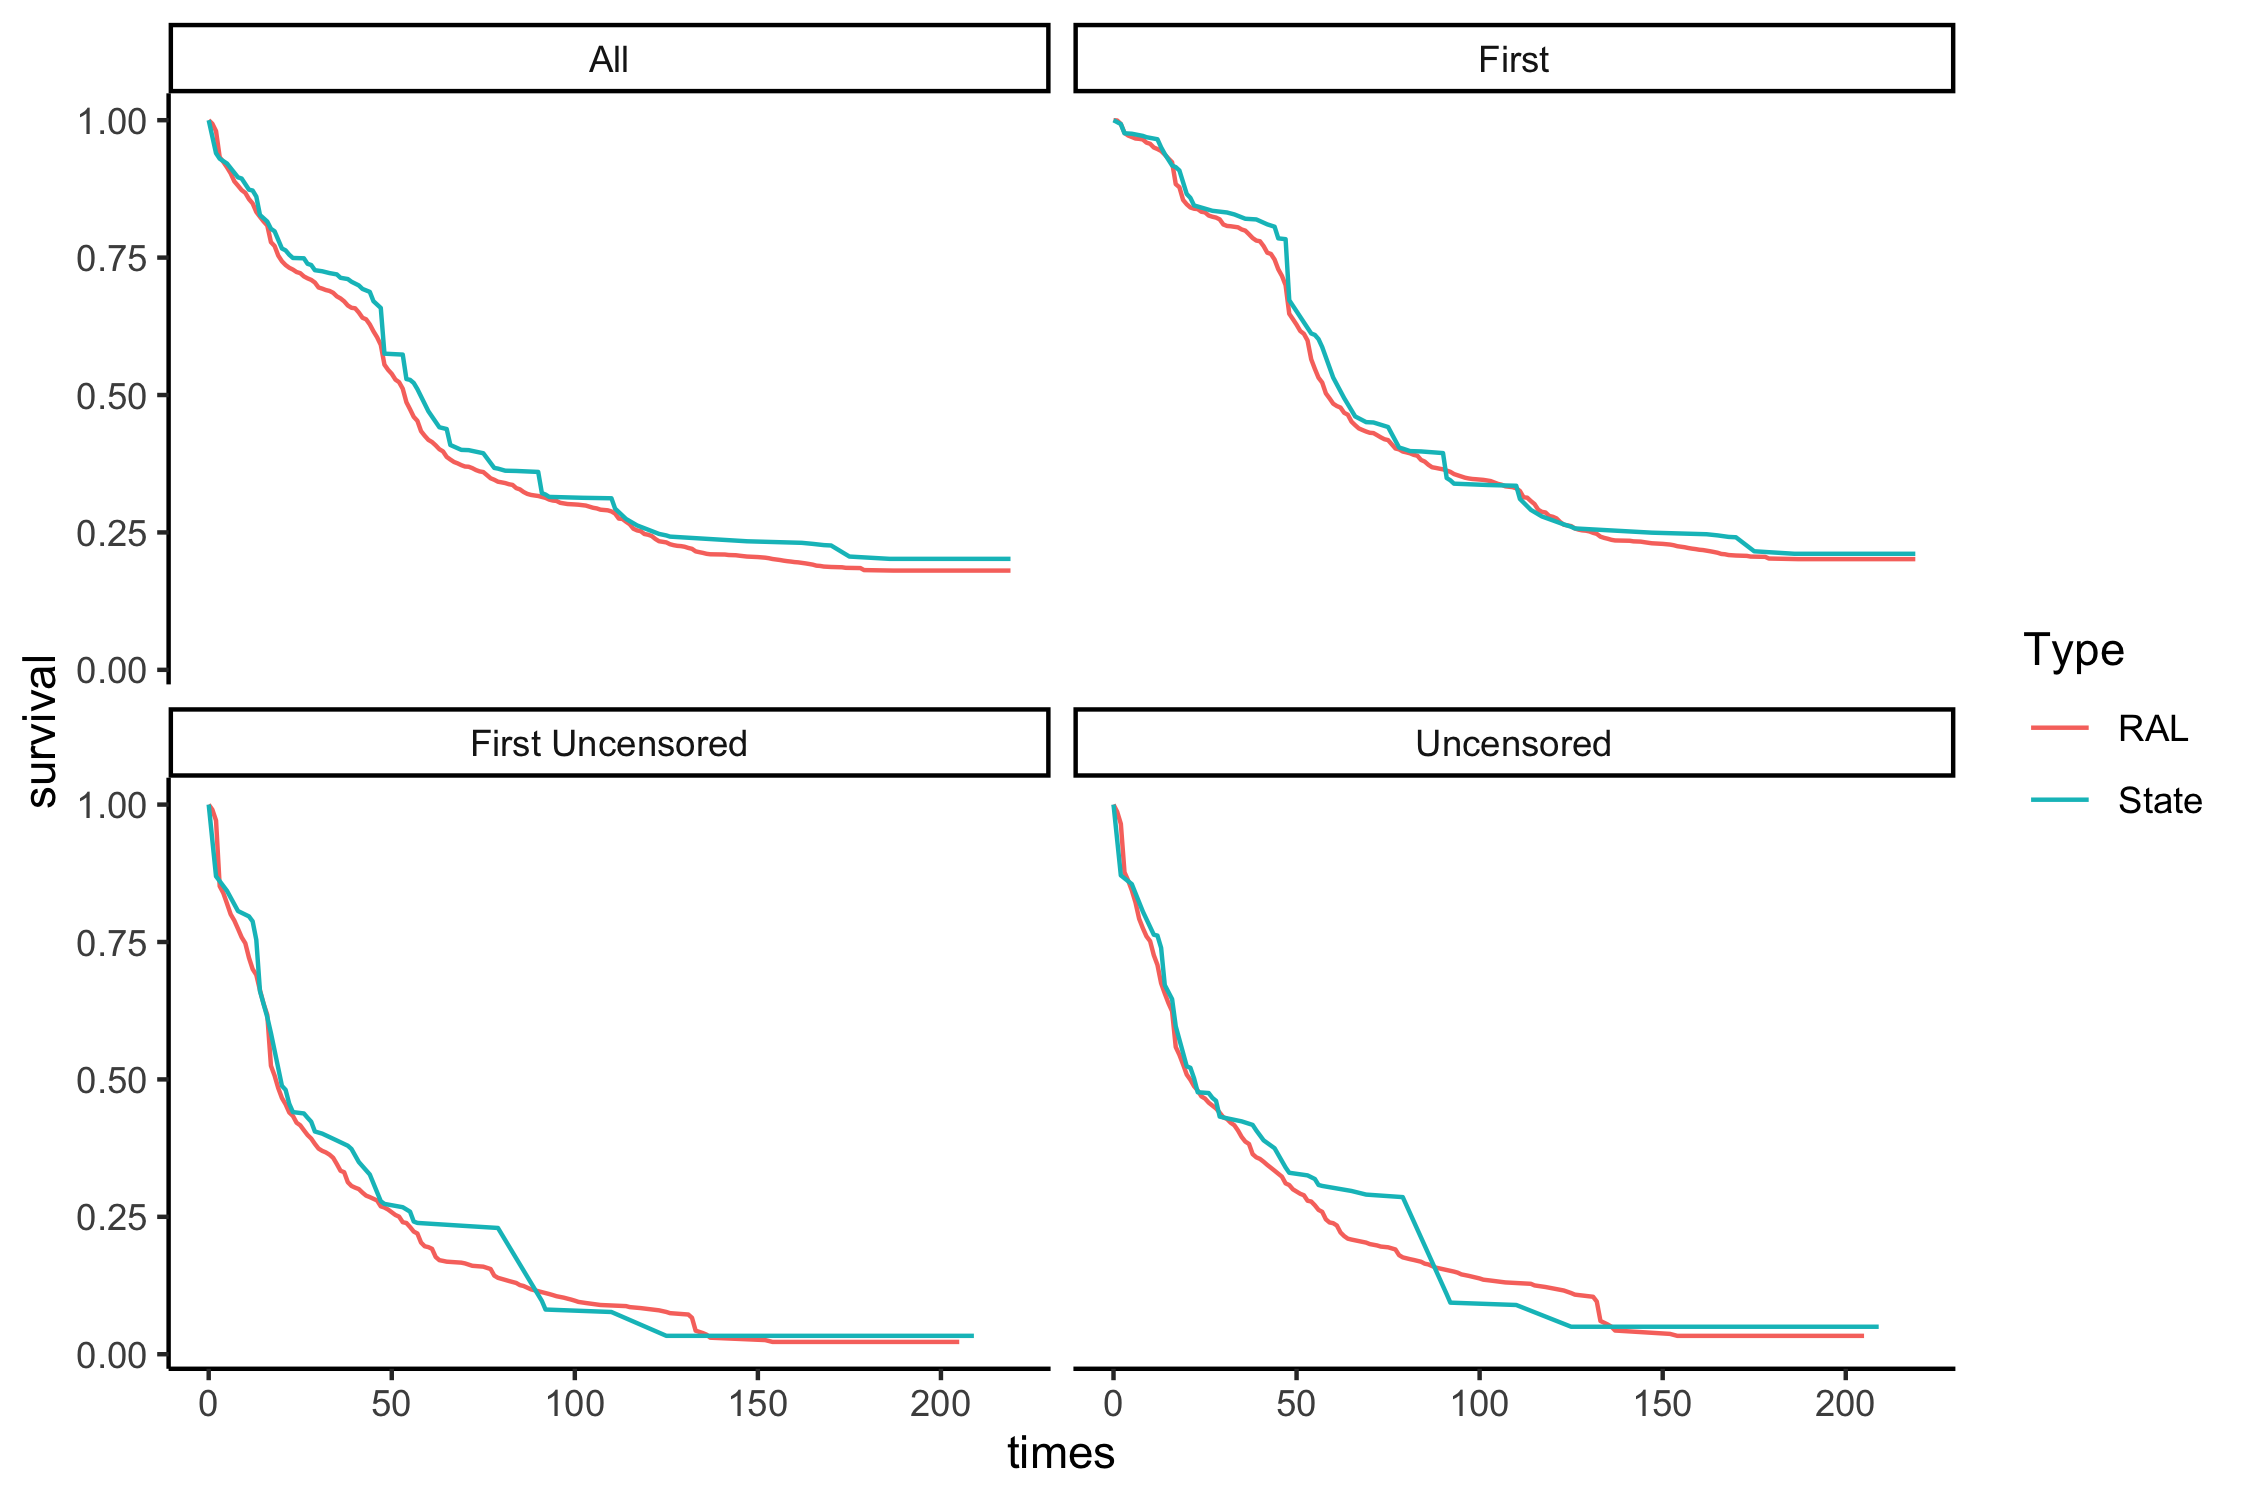
\includegraphics[width=1\textwidth]{../output/figures/ipwkm20.png}
\end{figure}

To formalize the test we have so far conducted visually, we compute adjusted log-rank tests of the hypothesis that two samples have the same hazard function, again informed by the ideas in \cite{xie2005adjusted}.  As in the adjusted survival curve estimates, the adjusted log-rank test weighs each observation by a propensity score.  \cite{xie2005adjusted} shows that as long as the propensity scores are consistently estimated, the adjusted log-rank test is distributed as standard normal, allowing us to use traditional asymptotic inference techniques.  Because we estimate our propensity scores using fixed effects in a high dimension non-linear model, we also compute p-values for these tests using the randomization inference technique recommended in \cite{xie2005adjusted}, as well as a standard non-parametric bootstrap.  Table \ref{tab:logrank} reports the test statistic values and p-values for the null hypothesis that the two survival curves are identical under each of these sample definitions, grid sizes, and inferential techniques.  There is no specification in which we can reject the null hypothesis under conventional significance thresholds that State and RAL unleased spells have the same survival function.  

\begin{table}[htbp]
	\begin{center}
		\begin{threeparttable}
			\caption{Log-Rank Tests of the Hypothesis That RAL and State Parcels Have Equally Long Unleased Spells}\label{tab:logrank}
			\small
			
\begin{tabular}{l>{\raggedleft\arraybackslash}p{8em}>{\raggedleft\arraybackslash}p{8em}>{\raggedleft\arraybackslash}p{8em}>{\raggedleft\arraybackslash}p{8em}}
\toprule
  & All & Uncensored & First & First Uncensored\\
\midrule
\addlinespace[0.3em]
\multicolumn{5}{l}{\textbf{Grid 10}}\\
\hspace{1em}statistic & -0.82 & -0.72 & -0.16 & -0.54\\
\hspace{1em}p.value & 0.41 & 0.47 & 0.87 & 0.59\\
\hspace{1em}ripval & 0.36 & 0.50 & 0.86 & 0.57\\
\hspace{1em}bspval & 0.42 & 0.47 & 0.88 & 0.60\\
\hspace{1em}N & 2,892 & 1,408 & 1,788 & 900\\
\addlinespace[0.3em]
\multicolumn{5}{l}{\textbf{Grid 20}}\\
\hspace{1em}statistic & 1.561 & 0.874 & 1.118 & 1.234\\
\hspace{1em}p.value & 0.119 & 0.382 & 0.263 & 0.217\\
\hspace{1em}ripval & 0.096 & 0.384 & 0.242 & 0.215\\
\hspace{1em}bspval & 0.152 & 0.389 & 0.263 & 0.213\\
\hspace{1em}N & 3,297. & 1,579. & 2,086. & 1,030.\\
\bottomrule
\end{tabular}

			\footnotesize
			\begin{tablenotes}
				\item ``Statistic'' is the log-rank statistic for the hypothesis that RAL and State parcels have equally long unleased spells.  Under the null hypothesis, this statistic is normally distributed with mean 0, and variance 1.  The first p-value compares this statistic to the quantiles of the standard normal distribution.  The second p-value (``ripval'') comes from a randomization inference procedure: randomly assign treatment according to the propensity scores, recompute the test statistic, and repeat 1000 times.  This p-value compres the original statistic to the distribution of the simulated statistics.  Finally, the third p-value, ``bspval'', comes from non-parametrically bootstrapping the entire testing process 1000 times and comparing the original statistic to its standardized bootstrap distribution.
				\item ``All'' refers to all unleased spells on on-shale PSF parcels since January 1, 2001.  ``Uncensored'' spells are the subset of those parcels which were already leased on January 1, 2001.  The date at which these spells begin is thus uncensored.  ``First'' spells are the subset of all spells which are the first unleased spell for a given parcel, and ``First Uncensored'' spells are the subset of uncensored spells which are the first unleased, uncensored spell for a given parcel.  Sample sizes differ in the top and bottom panels because the propensity score procedure will drop spells that lie in grids and/or time periods with either all RAL or all State leases, and grids of different sizes will result in a different number of dropped observations.
			\end{tablenotes}
		\end{threeparttable}
	\end{center}
\end{table}
	
\addtolength{\tabcolsep}{-6pt}

\subsection{RAL Lessor Heterogeneity}\label{app:lessor_hetero}
To document the extent to which different kinds of RAL lessors experience different leasing outcomes, we use lessor names to specify two notions of lessor sophistication.  First, we simply count how many leases a lessor has signed in recent history, going back to the year 2000.  Among all lessors who have signed an RAL lease overlying a shale formation since 2000, only 31\% signed more than one lease, 5\% signed five or more, and only 1\% signed 10 or more.  However, those highly experienced lessors signed many of the leases in our sample: 28\% of RAL leases are signed by lessors who have signed 5 or more since 2000, and 13\% are signed by lessors who have signed 10 or more.  It seems reasonable to expect that more experienced lessors employ more sophisticated negotiation tactics.  Second, we infer a lessor's sophistication from its name.  Lessors who are firms\footnote{We flag a lessor as a firm if its name contains one or more of the following strings: ``inc'', ``ltd'', ``llc', ``lp'', ``corp'', ``asset'', ``assoc'', ``company'', ``holdings'', ``partner'', or ``manag''.} and perhaps especially lessors that are firms explicitly working in the oil and gas business\footnote{We flag a lessor as working in the oil and gas business if its name contains one or more of the following strings: ``oil'', ``gas'', ``production'', ``explor'', ``mineral''.} may also employ more sophisticated negotiation tactics, so we generate flags for these two characteristics.  

We include dummy variables for each of these categories in our standard log bonus regressions, shown in Table \ref{tab:LessorHet}.  Across specifications, more experienced and/or more sophisticated lessors do seem to negotiate moderately higher bonus payments, but the differences are often imprecise, especially in the specifications that have 10-mile grid fixed effects. Moreover, while these lessors do better than novice negotiators, they still perform substantially worse than auctions. For example, consider specification 6, which uses 20-mile grid fixed effects and includes a dummy for lessors with 10 or more leases.  These lessors negotiate bonuses that are 10 log points higher than other RAL lessors, but since the average RAL lease has a bonus that is 54 log points lower than auctioned leases, this is still 44 log points lower than than the State's auction.

\addtolength{\tabcolsep}{5pt}
\begin{table}[H]
\begin{center}
\begin{threeparttable}
	\caption{RAL Lessor Heterogeneity and Bonus Payments}
	\label{tab:LessorHet}
 	\small
   	
\begin{tabular}{lcccccccc}
\toprule
 & ( 1 ) & ( 2 ) & ( 3 ) & ( 4 ) & ( 5 ) & ( 6 ) & ( 7 ) & ( 8 )\\
\midrule
 & 0.54 & 0.54 & 0.54 & 0.53 & 0.54 & 0.54 & 0.54 & 0.53\\

\multirow{-2}{*}{\raggedright\arraybackslash Auction} & (0.06) & (0.06) & (0.06) & (0.06) & (0.07) & (0.07) & (0.07) & (0.07)\\

 & 0.03 & \phantom{X} & \phantom{X} & \phantom{X} & 0.07 & \phantom{X} & \phantom{X} & \phantom{X}\\

\multirow{-2}{*}{\raggedright\arraybackslash LessorExperience5} & (0.04) & \phantom{X} & \phantom{X} & \phantom{X} & (0.03) & \phantom{X} & \phantom{X} & \phantom{X}\\

 & \phantom{X} & 0.07 & \phantom{X} & \phantom{X} & \phantom{X} & 0.10 & \phantom{X} & \phantom{X}\\

\multirow{-2}{*}{\raggedright\arraybackslash LessorExperience10} & \phantom{X} & (0.07) & \phantom{X} & \phantom{X} & \phantom{X} & (0.05) & \phantom{X} & \phantom{X}\\

 & \phantom{X} & \phantom{X} & 0.04 & \phantom{X} & \phantom{X} & \phantom{X} & 0.11 & \phantom{X}\\

\multirow{-2}{*}{\raggedright\arraybackslash LessorIsFirm} & \phantom{X} & \phantom{X} & (0.04) & \phantom{X} & \phantom{X} & \phantom{X} & (0.03) & \phantom{X}\\

 & \phantom{X} & \phantom{X} & \phantom{X} & 0.00 & \phantom{X} & \phantom{X} & \phantom{X} & 0.13\\

\multirow{-2}{*}{\raggedright\arraybackslash LessorIsEP} & \phantom{X} & \phantom{X} & \phantom{X} & (0.07) & \phantom{X} & \phantom{X} & \phantom{X} & (0.08)\\

\midrule
Grid & 10 & 10 & 10 & 10 & 20 & 20 & 20 & 20\\

Time & GY,Q & GY,Q & GY,Q & GY,Q & GY,Q & GY,Q & GY,Q & GY,Q\\

N & 1,515 & 1,515 & 1,515 & 1,515 & 1,515 & 1,515 & 1,515 & 1,515\\

$R^2$ & 0.961 & 0.961 & 0.961 & 0.961 & 0.945 & 0.945 & 0.945 & 0.945\\
\bottomrule
\end{tabular}
            
    \footnotesize
    \begin{tablenotes}
    	\item Regressions of the log of the bonus payment onto an auction indicator, as well as indicators for various measures of lessor sophistication.  LessorExperience5 refers to lessors who lease at least 5 times during 2000-2016, and LessorExperience10 requires 10 or more leases.  LessorIsFirm refers to lessors whose names suggest they are corporations, not natural people.  LessorIsEP refers to lessors whose names suggest they are experienced in the oil and gas industry.  All specifications include a spline in lease acres. 
    \end{tablenotes}
\end{threeparttable}
\end{center}
\end{table}

We also measure the extent to which the gap between auctioned and negotiated bonuses depends on the size of the lease. Our motivation for this analysis is that many of the actions involved with negotiating improved lease terms involve fixed costs which are invariant to the size of the lease. If the underlying value of a lease was exactly proportional to its size, then we might expect the owners of bigger leases to take more action to improve lease terms than the owners of smaller lessors do. Table \ref{tab:LeaseSizeHet} revisits the log bonus regressions from Table \ref{tab:table_main_bonus}. In column 1, we eschew our acres controls, project log bonus \textit{per acre} onto just a dummy for auction and grid-time fixed effects. Next we include an additional dummy for whether a negotiated lease is larger than the sample median size. Columns 2 and 5 show that under this constant returns to scale assumption (ie no spline in acres), big negotiated leases do pay a modest amount more than small negotiated leases. However, there are a variety of reasons to suspect that the underlying value of a lease is not proportional to size, since modern shale drilling requires large blocks of contiguous acreage to drill long horizontal wells and to efficiently co-locate surface equipment for many neighboring wells. Columns 3 and 6 re-introduce a spline in acres, as in the main specifications in the text. The results now show that negotiated leases above the median perform no better than those below the median, relative to the bonuses achieved at auction for each size group. 

\addtolength{\tabcolsep}{5pt}
\begin{table}[H]
\begin{center}
\begin{threeparttable}
	\caption{Lease Size Heterogeneity and Bonus Payments}
	\label{tab:LeaseSizeHet}
 	\small
   	
\begin{tabular}{lcccccc}
\toprule
 & ( 1 ) & ( 2 ) & ( 3 ) & ( 4 ) & ( 5 ) & ( 6 )\\
\midrule
 & 0.53 & 0.57 & 0.52 & 0.52 & 0.55 & 0.50\\

\multirow{-2}{*}{\raggedright\arraybackslash Auction} & (0.06) & (0.07) & (0.06) & (0.07) & (0.09) & (0.08)\\

 & \phantom{X} & 0.07 & -0.02 & \phantom{X} & 0.06 & -0.04\\

\multirow{-2}{*}{\raggedright\arraybackslash BigNegotiation} & \phantom{X} & (0.03) & (0.04) & \phantom{X} & (0.04) & (0.04)\\

\midrule
CRS & Yes & Yes & No & Yes & Yes & No\\

Estimate & G10Y & G10Y & G10Y & G20Y & G20Y & G20Y\\
\midrule

N & 1,515 & 1,515 & 1,515 & 1,515 & 1,515 & 1,515\\
\bottomrule
\end{tabular}
            
    \footnotesize
    \begin{tablenotes}
    	\item The variable ``BigNegotiation'' is equal to 1 if the lease is negotiated and if it is larger than the median negotiated lease, approximately \inputy{../output/estimates/negotiation_med_size.tex} acres; otherwise it is 0.  The dependent variable in the CRS specifications is the natural logarithm of bonus \textit{per acre}, while it is the natural logarithm of the bonus in the non-CRS specifications.  The non-CRS specifications in columns 3 and 6 include a spline in lease acres. All regressions include Grid10-Year or Grid20-Year fixed effects, and all include Year-Quarter fixed effects.
    \end{tablenotes}
\end{threeparttable}
\end{center}
\end{table}

This analysis provides a test of the hypothesis that the negotiations in this paper perform particularly badly because of the fact that RAL lessors only receive half of the proceeds they negotiate. In this sample, the average lease above the median is nearly five times larger than the average lease below the median. This implies that the differential incentive for effort across the two groups is much larger than the differential between RAL lessors and fully private lessors. Nevertheless, even in the CRS case, the maximum amount of the auction-negotiation gap that could be explained by shirking is small. Once we flexibly control for lease size, we find no evidence that large negotiated leases perform better than smaller negotiated leases. 

\pagebreak

\subsection{Lease-Parcel Comparison}\label{app:lease-parcel-decomp}
In this appendix, we present comparisons of lease level and parcel level regressions run on samples which are more immediately comparable than those presented in the main text. Table \ref{tab:lease_parcel_linear} presents linear results and \ref{tab:lease_parcel_Poisson} presents Poisson results. 

Columns 1-3 present lease level regressions, using 10 mile or 20 mile grid fixed effects, or DML spatial controls. Compared to the lease regressions presented in Section \ref{sec:ResultsLease}, we make two changes. First, we use the entire population of leases signed between 2004 and 2013. As described in Section \ref{sec:sampleSelection}, the main lease sample excludes RAL leases with features that do not overlap with auction leases, such as being too big or too small, or having multiple ownership interests. However, these lease level features are not defined at the parcel level. We thus include all leases when computing parcel level outcomes. Second, we discount all outcomes to 2004 (as opposed to the date the lease was signed). All models in Section \ref{sec:ResultsLease} include quarter of sample fixed effects, to account for large changes in fracking technology and oil prices over time. However, the parcel regressions are inherently cross-sectional. To facilitate comparison with the parcel regressions, we eschew all time controls here. 

Columns 4-6 present the corresponding parcel-level regressions. Compared to the results presented in Table \ref{tab:ParcelOutcomes}, there is only one change. Here we restrict the sample to parcels which sign at least one lease between 2004 and 2013, since these are the parcels underlying the lease sample in the first part of the table. 

Comparing across corresponding lease and parcel results reveals differences which are much smaller than the comparison discussed in Section \ref{sec:ParcelOutcomes}. In levels, the bonus results are slightly higher at the parcel level, while the output results are slightly lower. In logs, the bonus results are comparable, while the lease output and revenue results are twice as large. These small differences stem from two remaining factors which are fundamentally different across the two regressions: parcel vs. lease weighting and acreage controls. All models include a spline in acres. However leases may be much smaller or much bigger than their underlying parcel(s). When they are larger, a single transaction will receive more weight in the parcel regression than other transactions on single parcels. Conversely, re-leases of a parcel after expiration will receive \textit{less} weight in the parcel regression than in the lease regression, as will multiple concurrent smaller leases on a parcel. 

\addtolength{\tabcolsep}{-6pt}

\begin{table}[H]
\begin{center}
\begin{threeparttable}
	\caption{Lease Parcel Comparison: Linear Models}
	\label{tab:lease_parcel_linear}
 	\small
   	
\begin{tabular}{lcccccc}
\toprule
  & ( 1 ) & ( 2 ) & ( 3 ) & ( 4 ) & ( 5 ) & ( 6 )\\
\midrule
 & 0.354 & 0.394 & 0.352 & 0.515 & 0.558 & 0.491\\

\multirow{-2}{*}{\raggedright\arraybackslash Auction - Bonus} & (0.073) & (0.107) & (0.063) & (0.116) & (0.155) & (0.067)\\

\midrule
 & 0.425 & 0.457 & 0.469 & 0.243 & 0.384 & 0.299\\

\multirow{-2}{*}{\raggedright\arraybackslash Auction - Output} & (0.159) & (0.166) & (0.186) & (0.278) & (0.257) & (0.182)\\

\midrule
 & 1.699 & 1.784 & 1.916 & 0.794 & 1.329 & 1.396\\

\multirow{-2}{*}{\raggedright\arraybackslash Auction - Lease Revenue} & (0.597) & (0.683) & (0.712) & (1.084) & (1.048) & (0.677)\\

\midrule
 & 0.832 & 0.909 & 0.877 & 0.772 & 0.960 & 0.849\\

\multirow{-2}{*}{\raggedright\arraybackslash Auction - Seller Revenue} & (0.178) & (0.232) & (0.199) & (0.321) & (0.339) & (0.183)\\

\midrule
Estimate & G10 & G20 & DML & G10 & G20 & DML\\

Sample & All Leases & All Leases & All Leases & Leased Parcels & Leased Parcels & Leased Parcels\\

N & 2,389 & 2,389 & 2,389 & 1,784 & 1,784 & 1,784\\
\bottomrule
\end{tabular}
            
    \footnotesize
    \begin{tablenotes}
    	\item Outcomes are per acre and all models include a cubic spline in acres with 1 knot at the median lease or parcel size.  
    \end{tablenotes}
\end{threeparttable}
\end{center}
\end{table}

\begin{table}[H]
\begin{center}
\begin{threeparttable}
	\caption{Lease Parcel Comparison: Poisson Models}
	\label{tab:lease_parcel_Poisson}
 	\small
   	
\begin{tabular}{lcccccc}
\toprule
  & ( 1 ) & ( 2 ) & ( 3 ) & ( 4 ) & ( 5 ) & ( 6 )\\
\midrule
 & 0.716 & 0.777 & 0.717 & 0.690 & 0.729 & 0.644\\

\multirow{-2}{*}{\raggedright\arraybackslash Auction - Bonus} & (0.109) & (0.128) & (0.075) & (0.088) & (0.110) & (0.053)\\

\midrule
 & 0.520 & 0.691 & 0.425 & 0.218 & 0.350 & 0.198\\

\multirow{-2}{*}{\raggedright\arraybackslash Auction - Output} & (0.152) & (0.153) & (0.171) & (0.154) & (0.112) & (0.114)\\

\midrule
 & 0.509 & 0.653 & 0.430 & 0.189 & 0.332 & 0.200\\

\multirow{-2}{*}{\raggedright\arraybackslash Auction - Lease Revenue} & (0.148) & (0.168) & (0.166) & (0.140) & (0.129) & (0.112)\\

\midrule
 & 0.608 & 0.696 & 0.526 & 0.370 & 0.470 & 0.350\\

\multirow{-2}{*}{\raggedright\arraybackslash Auction - Seller Revenue} & (0.101) & (0.116) & (0.105) & (0.087) & (0.090) & (0.063)\\

\midrule
Estimate & G10 & G20 & DML & G10 & G20 & DML\\

Sample & All Leases & All Leases & All Leases & Leased Parcels & Leased Parcels & Leased Parcels\\

N & 2,389 & 2,389 & 2,389 & 1,784 & 1,784 & 1,784\\
\bottomrule
\end{tabular}
            
    \footnotesize
    \begin{tablenotes}
    	\item Outcomes are in levels and all models include a cubic spline in acres with 1 knot at the median lease or parcel size.  
    \end{tablenotes}
\end{threeparttable}
\end{center}
\end{table}

\section{Data Cleaning \label{sec:DataCleaning}}

\subsection{Sample construction \label{sec:AppendixSampleConstruction}}

Table \ref{tab:waterfall} presents the number of negotiated and auctioned leases existing in original data provided to us by GLO, as well as the subset that survives each of our sample restrictions. We begin with the universe of GLO leases signed between 2004 and 2016 that can be matched to original PSF parcels and have non-missing lease characteristics.  We first drop leases on PSF land types other than Relinquishment Act land or belonging entirely to the GLO.  Next, we use the EIA's definition of shale formations in Texas, shown shaded in yellow in Figure \ref{fig:RAL_map}, to drop leases on land that does not overlie a shale formation.  To ensure a comparable distribution of lease covariates, we drop especially small leases, especially large leases, and leases with especially short primary terms.  We drop leases on ``undivided'' mineral interests, which occur when two or more parties share ownership of the surface and or mineral estate.\footnote{For example, if parents John and Mary bequeath their 640 acre parcel to their two children, Bob and Jane, then Bob and Jane each have an undivided interest in the parcel.  In principal, it is possible for Bob and Jane to separately lease their respective undivided interests to different oil and gas companies.} We drop a small number of leases on non-RAL land that are allocated via bilateral negotiation specifically because only one party can economically use the land.   Similarly, we drop RAL leases that are allocated by auction when the State is unable to determine who the rightful surface owner is.  Finally, we drop non-standard negotiated agreements between the State of Texas and E\&P companies that do not have the traditional mineral lease contract structure.

\begin{table}[H]
	\begin{center}
	\begin{threeparttable}
		\caption{Sample Construction}
		\label{tab:waterfall}
		\small
		
\begin{tabular}{llrr}
\toprule
 & Drop Reason & Negotiation & Auction\\
\midrule
Initial Sample &  & 4,828 & 827\\
 & Not RAL or State lease & 4,368 & 786\\
 & Not on Shale & 2,517 & 553\\
 & Less Than 10 or Greater Than 1,000 Acres & 1,985 & 499\\
 & Gross and Net Acreage Differ & 1,658 & 497\\
 & Undivided Interest & 1,092 & 493\\
 & Term Less Than 1 Year & 1,073 & 493\\
 & Negotiated State Lease & 1,066 & 493\\
 & Auctioned RAL Lease & 1,066 & 454\\
 & Nonstandard Lease Category & 1,061 & 454\\
Final Sample &  & 1,061 & 454\\
\bottomrule
\end{tabular}
            
		\footnotesize
		\begin{tablenotes}
			\item Additional discussion provided in Section \ref{sec:sampleSelection}.
		\end{tablenotes}
	\end{threeparttable}
	\end{center}
\end{table}

\subsection{Firm Names \label{sec:FirmNameCleaning}}
Though we observe the name of the firm on the lease, E\&P companies sometimes use intermediaries, or ``landmen,'' to acquire land, and, in these cases, we might not observe the relevant firm. One reason why a firm would do this would be to prevent its competitors from discovering its interest in a particular play before it had had acquired enough land to develop it. This ``secrecy'' motivation is probably relevant, because the presence of non-E\&P company lessees is much more common in the auction data than in the negotiated data. This is perhaps not surprising, since the auction records are publicly released shortly after the auction, and easily observable.  To partially overcome this challenge, we use data on \textit{lease assignments}, legal transactions which formally change ownership of a lease from one firm to another, to better infer who the ultimate E\&P company is on leases initially awarded to non-E\&P company lessees. We observe assignments on 18\% of RAL leases and 33\% of auction leases. For each non-E\&P company in our data who ever assigns a lease to an E\&P company, we identify a variety of ``most common'' assignees, using auction status, location and time.  For non-E\&P company leases in which we do not observe an assignment, we characterize the ``real'' lessee as this (conditional) most common assignee.  Though this process is not perfect, it does greatly reduce the number of leases that we believe are allocated to lessees that are not E\&P companies.

\pagebreak

\section{Double/Debiased Machine Learning Estimation Details}\label{sec:dml}

To non-parametrically control for the effects of location and time on lease terms and lease outcomes, we adopt the double/debiased machine learning framework of \cite{chernozhukov2018double}, which we refer to as ``DML'' models.  In our partially linear DML models, we use the partially linear model derived in equation 4.4 of that paper.  In our pseudo-Poisson models, we derive a Neyman-orthogonal score for pseudo-Poisson regression, documented below.  

In all DML models, we implement the nuisance parameter estimation with random forests, using the \texttt{regression\_forest} function from the \texttt{grf} package for the R language, as described in \cite{athey2019generalized}, with 1000 trees per forest.  Following the suggestions in \cite{chernozhukov2018double}, we construct a single point estimate and covariance matrix of the relevant parametric terms using 5-fold cross-fitting, and report the ``median'' values of these across 101 randomized cross-fitted partitions, as in definition 3.3 of that paper. 

To derive the Neyman-orthogonal moment for pseudo-Poisson regression, we closely follow the discussion following Lemma 2.5 of \cite{chernozhukov2018double}.  Let $Y$ be a non-negative outcome, $D$ a \textit{binary} covariate, and $X$ a vector of controls that we wish to model non-parametrically, like location, time and lease or parcel size.  Our goal is to pick the values of $\theta$ and $\beta(X)$ that minimize a pseudo-Poisson quasi-log-likelihood criteria:
\begin{equation*}
	(\theta_0, \beta(X)_0) = \arg \max_{\theta, \beta(X)} \mathbb{E}\left[Y(D\theta + \beta(X))-\exp(D\theta + \beta(X))\right]
\end{equation*}

Let $\beta_{\theta}(x)$ be the best fitting value of $\beta(x)$ for a given value of $\theta$.  For the above criterion, we can find this implicitly by setting the gradient of the \textit{conditional} expectation of the criterion with respect to $\beta(x)$ equal to 0, and re-arranging terms:
\begin{equation*}
	\exp(\beta_{\theta}(x)) = \frac{\gamma(x)}{\exp(\theta)\delta(x) + 1 - \delta(x)}
\end{equation*}	
where $\gamma(x) = \mathbb{E}\left[Y\mid X = x\right]$ and $\delta(x) = \mathbb{E}\left[D\mid X = x\right]$.  The Neyman-orthogonal moment for pseudo-Poisson regression is the total derivative of the quasi-log-likelihood criterion with respect to $\theta$, after we plug in the solution for $\exp(\beta_{\theta}(x))$:
\begin{equation*}
	\psi(Y, D, X; \theta, \gamma(x), \delta(x)) = \left(Y-\frac{\exp(D\theta)\gamma(X)}{\exp(\theta)\delta(X) + 1 - \delta(X)}\right)\left(D - \frac{\exp(\theta)\delta(X)}{\exp(\theta)\delta(X) + 1 - \delta(X)}\right).
\end{equation*}
This is the objective whose empirical average we set to 0 in our pseudo-Poisson regressions.

\section{Empirical Auction Analysis Details}\label{sec:AppendixAuction}

We estimate the distribution of bidder values, conditional on observable and unobservable auction-level heterogeneity, in the independent private values framework\footnote{Though \textit{offshore} mineral leasing has long been studied in the common values framework (e.g., \cite{hendricks_empirical_1988}, most recent analysis of \textit{onshore} mineral lease auctions takes place in the private values framework.  \cite{kong2016sequential} and \cite{kong_selective_2017} both provide informative discussions about why private values make sense in studying the recent shale boom.}, by following the model in \cite{roberts2013unobserved}.  The first step is to regress the natural logarithm of an auction's reserve price $R$, in nominal dollars per acre, on a cubic spline in its size in acres $f(A)$, and fixed effects for the tract's county $\delta_{c}$ and the date the auction took place $\gamma_{t}$.
\begin{equation*}
	\log R_i = f(A_i) + \delta_{c(i)} + \gamma_{t(i)} + \epsilon_i
\end{equation*}
We define the observed heterogeneity index as the predicted value from this regression, $H_i = \widehat{f}(A_i) + \widehat{\delta}_{c(i)} + \widehat{\gamma}_{t(i)}$, and the unobserved heterogeneity index as $U_i = \log R_i - H_i$, the residual.  We estimate this model on the entire population of GLO auctions for tracts in counties that overlap shale formations, during 2004-2016, including auctions that do not receive any bids at or above the reserve price.

Next, we use $(H_i,U_i)$ as the heterogeneity covariates in the procedure specified in section 4 of \cite{guerre2000optimal}.  After recovering the bidder values that are consistent with equilibrium bidding, we find that the bid-value relationship is occasionally non-monotonic.  When this occurs, we follow the advice in \cite{chernozhukov2009improving} and re-order estimated values within an auction to guarantee monotonicity.

Table \ref{tab:AuctionNBidsRobust} shows how our key auction statistics are sensitive to different kernel bandwidth choices, dropping bids near the boundary of the support of the distribution of bids and/or heterogeneity covariates, and dropping auctions where value re-arrangement is necessarily to maintain monotonicity of the bid-value relationship.
\addtolength{\tabcolsep}{4pt}
\begin{table}[H]
\begin{center}
\begin{threeparttable}
	\caption{Auction Robustness}
	\label{tab:AuctionNBidsRobust}
 	\small
   	
\begin{tabular}{lcc>{\centering\arraybackslash}p{7em}>{\centering\arraybackslash}p{7em}}
\toprule
Sample & Bandwidth Scaling & Auctions & Average 1-to-2 Markup & Average 1-to-2 Allocative Gain\\
\midrule
All & 0.5 & 202 & 0.34 & 0.41\\
All & 1.0 & 202 & 0.34 & 0.47\\
All & 2.0 & 202 & 0.34 & 0.58\\
Drop Trimmed & 1.0 & 154 & 0.32 & 0.40\\
Drop Rearranged & 1.0 & 162 & 0.36 & 0.49\\
Drop Trimmed and Rearranged & 1.0 & 117 & 0.34 & 0.41\\
\bottomrule
\end{tabular}
            
    \footnotesize
    \begin{tablenotes}
    	\item This table summarizes bids from GLO auctions with 2 or more bidders across various assumptions made in the GPV analysis.  The sample includes all auctions in the first three rows.  In the fourth row we drop auctions where one or more bids would be trimmed under the GPV trimming rules.  In the fifth row we drop auctions where the estimated pseudovalues are not monotonic in the bids.  In the sixth row, we drop auctions where bids would be either trimmed or pseudovalues would need to be rearranged to impose monotonicity. ``Bandwidth Scaling'' refers to whether we use the Silverman rule for bandwidth selection (1.0) or half (0.5) or twice (2.0) the Silverman rule. The ``1-to-2 Markup'' is the natural logarithm of the ratio of the winning bid to the second highest bid.  The ``1-to-2 Allocative Gain'' is the natural logarithm of the ratio of the GPV pseudovalues of the winning and second highest bids.
    \end{tablenotes}
\end{threeparttable}
\end{center}
\end{table}

\pagebreak

\section{RAL Lease Addenda}\label{sec:Appendix_Addenda}
In addition to specifying bonus payments, royalty rates and primary terms, mineral leases also specify how the contracting parties will resolve disagreements about issues related to environmental impact, on-site water usage, and surface property disruptions, among other things.  These protective clauses are standardized in the GLO auction lease agreement, and there are ``default'' values for them in the GLO's required RAL lease agreement.  However, RAL surface owners and their contracting partners can optionally negotiate some deviations from the standard lease.  To the extent that RAL surface owners are willing to forego up-front bonus payments for stricter surface protections during subsequent exploration and production, we might be worried that the differences in bonus payments that we observe are not caused by the mechanism itself, but rather by a compensating differentials story.  

It is important to note that it is not possible to directly condition on the content of these protective clauses and maintain our causal interpretation of the differences between auctioned and negotiated leases, for the same reason that we do not condition on royalty rates and primary terms.  See the discussion at the end of Section \ref{sec:ResultsLease}.  However, having recognized the challenge in interpreting these results as causal, we explore the extent to which RAL lease addenda content affects our regression estimates.

To do this, we had a team of research assistants do a dual-entry review of the text of these lease addenda for all RAL leases signed between 2005 and 2016.  They characterized the extent to which each one improved or deteriorated the surface owner's rights along dimensions such as environmental impact, water usage, and surface property disruptions, guided by the procedure in \cite{vissing_one--many_2017}.  About 73\% of RAL leases have one or more additional clauses in their lease addenda.  In Table \ref{tab:table_bonus_addenda}, we include measures of these protective clauses in bonus and output regressions like those shown in Table \ref{tab:table_main_bonus} and \ref{tab:output_stacked}.  The first two columns mirror the result shown in the main text: auctioned pleases pay 50 or more log points in up-front bonus payments than negotiated leases do, and output is similarly higher.  In the next two columns, we include covariates which measure the number of pages in an RAL lease's addendum, as well as the number of specific legal clauses documented.  Finally, in the last two columns we include covariates for each specific kind of clause that occur in these addenda, coded as $-1$ if a lease's addenda deteriorates the surface owner's rights, relative to the standard RAL lease, $0$ if it is absent or does not affect the surface owner's rights, and $+1$ if it improves upon the surface owner's rights.  Across all specifications, we find no evidence that variation between auctioned and negotiated leases in protective clauses can ``explain away'' the observed differences in both bonus payments and output. 

\begin{table}[H]
\begin{center}
\begin{threeparttable}
	\caption{Bonus Payments, Lease Output, and Mechanism Type: Robustness to RAL Lease Addenda}
	\label{tab:table_bonus_addenda}
 	\small
   	
\begin{tabular}{lcccccc}
\toprule
  & ( 1 ) & ( 2 ) & ( 3 ) & ( 4 ) & ( 5 ) & ( 6 )\\
\midrule
 & 0.57 & 0.65 & 0.61 & 0.80 & 0.61 & 0.70\\

\multirow{-2}{*}{\raggedright\arraybackslash Auction - log(Bonus)} & (0.06) & (0.05) & (0.06) & (0.07) & (0.06) & (0.06)\\

N & 1,409 & 1,409 & 1,409 & 1,409 & 1,409 & 1,409\\

\midrule
 & 1.10 & 1.39 & 1.23 & 1.66 & 1.16 & 1.32\\

\multirow{-2}{*}{\raggedright\arraybackslash Auction - Output} & (0.34) & (0.44) & (0.42) & (0.52) & (0.43) & (0.44)\\

N & 1,153 & 1,153 & 1,153 & 1,153 & 1,153 & 1,153\\

\midrule
Addenda Controls & None & None & Pages + Clauses & Pages + Clauses & Individual & Individual\\

Grid & 10 & DML & 10 & DML & 10 & DML\\

Time & GY,Q & DML & GY,Q & DML & GY,Q & DML\\
\bottomrule
\end{tabular}
            
    \footnotesize
    \begin{tablenotes}
    	\item Columns 1 and 2 report baseline specifications with no controls RAL lease addenda content.  We measure lease addenda content in columns 3 and 4 using the number of pages and number of individual clauses in the addenda.  In Columns 5 and 6, we include a set of individual dummy variables indicating whether the addenda improves (+1), deteriorates (-1) or is similar to the standard auction lease (0) along each of these margins: Surface Protection, Payment Terms, Location Requirements, Pugh Clause, Cleanup Terms, Livestock Protection, On-site Water Use, Waste Management, Definitional Changes, Pollution Protection, Infrastructure Constraints, Caliche Use, Additional Fees, Time Constraints, Miscellaneous. Columns 1, 3, and 5 control for space and time using 10-mile grid by year of sample fixed effects, as well as fixed effects for quarter of sample.  Columns 2, 4, and 6 use a double/debiased machine learning routine, as recommended in \cite{chernozhukov2018double}, with non-parametric controls for lease latitude, longitude, effective date, size and addenda measures.  Sample includes leases signed between 2005-2016.
    \end{tablenotes}
\end{threeparttable}
\end{center}
\end{table}

\end{appendices}
\bibliographystyle{econ}
\bibliography{cs_texas}

\end{document}



